\documentclass[11pt,a4paper]{article}

\usepackage{amsmath}
\usepackage{epsfig}
\usepackage{multicol}
\usepackage{natbib}




\usepackage[toc,page]{appendix}
\usepackage{amsmath, amssymb}
\usepackage{bm}% bold math
\usepackage{cancel, caption}
\usepackage{dcolumn}% Align table columns on decimal point
\usepackage{epsfig, epsf}
\usepackage{graphicx,fancyhdr,natbib,subfigure}
\usepackage{lscape, longtable}
\usepackage{hyperref,ifthen}
\usepackage{verbatim}
\usepackage{color}
\usepackage[usenames,dvipsnames]{xcolor}
\usepackage{listings}
%% http://en.wikibooks.org/wiki/LaTeX/Colors



%%%%%%%%%%%%%%%%%%%%%%%%%%%%%%%%%%%%%%%%%%%
%       define Journal abbreviations      %
%%%%%%%%%%%%%%%%%%%%%%%%%%%%%%%%%%%%%%%%%%%
\def\nat{Nat} \def\apjl{ApJ~Lett.} \def\apj{ApJ}
\def\apjs{ApJS} \def\aj{AJ} \def\mnras{MNRAS}
\def\prd{Phys.~Rev.~D} \def\prl{Phys.~Rev.~Lett.}
\def\plb{Phys.~Lett.~B} \def\jhep{JHEP} \def\nar{NewAR}
\def\npbps{NUC.~Phys.~B~Proc.~Suppl.} \def\prep{Phys.~Rep.}
\def\pasp{PASP} \def\aap{Astron.~\&~Astrophys.} \def\araa{ARA\&A}
\def\jcap{\ref@jnl{J. Cosmology Astropart. Phys.}}%
\def\physrep{Phys.~Rep.}

\newcommand{\preep}[1]{{\tt #1} }

%%%%%%%%%%%%%%%%%%%%%%%%%%%%%%%%%%%%%%%%%%%%%%%%%%%%%
%              define symbols                       %
%%%%%%%%%%%%%%%%%%%%%%%%%%%%%%%%%%%%%%%%%%%%%%%%%%%%%
\def \Mpc {~{\rm Mpc} }
\def \Om {\Omega_0}
\def \Omb {\Omega_{\rm b}}
\def \Omcdm {\Omega_{\rm CDM}}
\def \Omlam {\Omega_{\Lambda}}
\def \Omm {\Omega_{\rm m}}
\def \ho {H_0}
\def \qo {q_0}
\def \lo {\lambda_0}
\def \kms {{\rm ~km~s}^{-1}}
\def \kmsmpc {{\rm ~km~s}^{-1}~{\rm Mpc}^{-1}}
\def \hmpc{~\;h^{-1}~{\rm Mpc}} 
\def \hkpc{\;h^{-1}{\rm kpc}} 
\def \hmpcb{h^{-1}{\rm Mpc}}
\def \dif {{\rm d}}
\def \mlim {m_{\rm l}}
\def \bj {b_{\rm J}}
\def \mb {M_{\rm b_{\rm J}}}
\def \mg {M_{\rm g}}
\def \qso {_{\rm QSO}}
\def \lrg {_{\rm LRG}}
\def \gal {_{\rm gal}}
\def \xibar {\bar{\xi}}
\def \xis{\xi(s)}
\def \xisp{\xi(\sigma, \pi)}
\def \Xisig{\Xi(\sigma)}
\def \xir{\xi(r)}
\def \max {_{\rm max}}
\def \gsim { \lower .75ex \hbox{$\sim$} \llap{\raise .27ex \hbox{$>$}} }
\def \lsim { \lower .75ex \hbox{$\sim$} \llap{\raise .27ex \hbox{$<$}} }
\def \deg {^{\circ}}
%\def \sqdeg {\rm deg^{-2}}
\def \deltac {\delta_{\rm c}}
\def \mmin {M_{\rm min}}
\def \mbh  {M_{\rm BH}}
\def \mdh  {M_{\rm DH}}
\def \msun {M_{\odot}}
\def \z {_{\rm z}}
\def \edd {_{\rm Edd}}
\def \lin {_{\rm lin}}
\def \nonlin {_{\rm non-lin}}
\def \wrms {\langle w_{\rm z}^2\rangle^{1/2}}
\def \dc {\delta_{\rm c}}
\def \wp {w_{p}(\sigma)}
\def \PwrSp {\mathcal{P}(k)}
\def \DelSq {$\Delta^{2}(k)$}
\def \WMAP {{\it WMAP \,}}
\def \cobe {{\it COBE }}
\def \COBE {{\it COBE \;}}
\def \HST  {{\it HST \,\,}}
\def \Spitzer  {{\it Spitzer \,}}
\def \ATLAS {VST-AA$\Omega$ {\it ATLAS} }
\def \BEST   {{\tt best} }
\def \TARGET {{\tt target} }
\def \TQSO   {{\tt TARGET\_QSO}}
\def \HIZ    {{\tt TARGET\_HIZ}}
\def \FIRST  {{\tt TARGET\_FIRST}}
\def \zc {z_{\rm c}}
\def \zcz {z_{\rm c,0}}

\newcommand{\ltsim}{\raisebox{-0.6ex}{$\,\stackrel
        {\raisebox{-.2ex}{$\textstyle <$}}{\sim}\,$}}
\newcommand{\gtsim}{\raisebox{-0.6ex}{$\,\stackrel
        {\raisebox{-.2ex}{$\textstyle >$}}{\sim}\,$}}
\newcommand{\simlt}{\raisebox{-0.6ex}{$\,\stackrel
        {\raisebox{-.2ex}{$\textstyle <$}}{\sim}\,$}}
\newcommand{\simgt}{\raisebox{-0.6ex}{$\,\stackrel
        {\raisebox{-.2ex}{$\textstyle >$}}{\sim}\,$}}

\newcommand{\Msun}{M_\odot}
\newcommand{\Lsun}{L_\odot}
\newcommand{\lsun}{L_\odot}
\newcommand{\Mdot}{\dot M}

\newcommand{\sqdeg}{deg$^{-2}$}
\newcommand{\lya}{Ly$\alpha$\ }
%\newcommand{\lya}{Ly\,$\alpha$\ }
\newcommand{\lyaf}{Ly\,$\alpha$\ forest}
%\newcommand{\eg}{e.g.~}
%\newcommand{\etal}{et~al.~}
\newcommand{\lyb}{Ly$\beta$\ }
\newcommand{\cii}{C\,{\sc ii}\ }
\newcommand{\ciii}{C\,{\sc iii}]\ }
\newcommand{\civ}{C\,{\sc iv}\ }
\newcommand{\SiIV}{Si\,{\sc iv}\ }
\newcommand{\mgii}{Mg\,{\sc ii}\ }
\newcommand{\feii}{Fe\,{\sc ii}\ }
\newcommand{\feiii}{Fe\,{\sc iii}\ }
\newcommand{\caii}{Ca\,{\sc ii}\ }
\newcommand{\halpha}{H\,$\alpha$\ }
\newcommand{\hbeta}{H\,$\beta$\ }
\newcommand{\hgamma}{H\,$\gamma$\ }
\newcommand{\hdelta}{H\,$\delta$\ }
\newcommand{\oi}{[O\,{\sc i}]\ }
\newcommand{\oii}{[O\,{\sc ii}]\ }
\newcommand{\oiii}{[O\,{\sc iii}]\ }
\newcommand{\heii}{[He\,{\sc ii}]\ }
\newcommand{\nv}{N\,{\sc v}\ }
\newcommand{\nev}{Ne\,{\sc v}\ }
\newcommand{\neiii}{[Ne\,{\sc iii}]\ }
\newcommand{\aliii}{Al\,{\sc iii}\ }
\newcommand{\siiii}{Si\,{\sc iii}]\ }


%%%%%%%%%%%%%%%%%%%%%%%%%%%%%%%%%%%%%%%%%%%%%%%%%%%%%
%              define Listings                       %
%%%%%%%%%%%%%%%%%%%%%%%%%%%%%%%%%%%%%%%%%%%%%%%%%%%%%
\definecolor{dkgreen}{rgb}{0,0.6,0}
\definecolor{gray}{rgb}{0.5,0.5,0.5}
\definecolor{mauve}{rgb}{0.58,0,0.82}

\lstset{frame=tb,
  language=Python,
  aboveskip=3mm,
  belowskip=3mm,
  showstringspaces=false,
  columns=flexible,
  basicstyle={\small\ttfamily},
  numbers=none,
  numberstyle=\tiny\color{gray},
  keywordstyle=\color{blue},
  commentstyle=\color{dkgreen},
  stringstyle=\color{mauve},
  breaklines=true,
  breakatwhitespace=true,
  tabsize=3
}

\begin{document}

\title{SEDs, $f_{\nu}$ and $f_{\lambda}$'s}
\author{Nic ``What Have I got wrong here'' Ross}
\date{\today}
\maketitle


% Usually omit these for ApJ or MNRAS style files:
%\tableofcontents
%\listoffigures
%\listoftables

\begin{abstract}
%{\bf The} definitive document, 
``README'' and ``Cheat Sheet'' to SEDs, $f_{\nu}$ and $f_{\lambda}$
and all that carry-on...
\end{abstract}



\clearpage
\section{Definitions, terms and Units}
Starting off with just some basic definitions, terms and units. A big
push here will be to be consistent and also as comprehensive as
possible.

\begin{table*}
  \begin{center}
    \setlength{\tabcolsep}{4pt}
    \begin{tabular}{llllr}
      \hline
      \hline
      Physical Quantity & symbol & Unit name & Units & e.g. $\log$(OoM)   \\
      \hline
      spectral flux density$^{a}$ &  $f_{\nu}$        &             & W                  m$^{-2}$ Hz$^{-1}$                      & -27 -- -35 \\
      spectral flux density          &  $f_{\nu}$        & Janksy  & W                   m$^{-2}$ Hz$^{-1}$  $10^{-26}$   & $\mu$ to 10's of milli \\
      spectral flux density          &  $f_{\nu}$        &             & erg s$^{-1}$ cm$^{-2}$ Hz$^{-1}$                      & -24 -- -32 \\
      spectral flux density          &  $f_{\nu}$        & Jansky  & erg s$^{-1}$ cm$^{-2}$ Hz$^{-1}$  $10^{-23}$   & $\mu$ to 10's of milli \\
      spectral flux density          &  $f_{\lambda}$  &             &  W                  m$^{-2}$ m$^{-1}$                       &  \\
      spectral flux density          &  $f_{\lambda}$  &             &  W                  m$^{-2}$ $\mu$m$^{-1}$             &  \\
                                                &                       &             &                        & \\
      $^{a}$energy density         & $\nu f_{\nu}$   &  erg s$^{-1}$ cm$^{-2}$       &        & -12 -- -16 \\
     $^{b}$ --                            & $\nu F_{\nu}$ &                                            &        &      \\
                                                &                       &             &                        & \\
     $^{c}$ --                            &        $L_{\nu}$ &  erg s$^{-1}$ Hz$^{-1}$       &        &    26 -- 34  \\
                                                &                       &             &                        & \\

     $^{a}$Luminosity              &  $\nu L_{\nu}$ &  erg s$^{-1}$                        &       &   43 -- 47 \\
     $^{a}$Luminosity              &  $L$ &  erg s$^{-1}$                        &       &   43 -- 47 \\
      \hline
      \hline
   \end{tabular}
    \caption{$^{a}$see e.g. Fig. 10 of \citet{Richards06b}.\\
      $^{b}$e.g. URL [1]\\
      $^{c}$e.g. Bourne et al. (2011)
}
     \label{tab:units_overview}
  \end{center}
\end{table*}



\clearpage
\begin{landscape} 
\begin{table*}
  \begin{center}
    \setlength{\tabcolsep}{4pt}
%    \begin{tabular}{l l l l l l}
    \begin{tabular}{  p{45mm}   p{20mm}  p{40mm}  p{20mm}   p{20mm}  p{90mm}} 
      \hline
      \hline
      Name	                                      & Symbol                       & Unit name                     & Unit symbol  & Dimension                 & Notes   \\
      \hline
      Radiant energy	                      &  $Q_{\rm e}$                 & Joule                              &	J             & M L$^{2}$    T$^{-2}$     & Energy of electromagnetic radiation. \\
      Radiant energy density            & w$_{\rm e}$	             & Joule per cubic metre    & J/m$^3$	      & M L$^{-1}$  T$^{-2}$     & Radiant energy per unit volume. \\
      Radiant flux                             & $\phi_{\rm e}$              & Watt	                              & W = J/s         & M L$^{2}$    T$^{-3}$    & Radiant energy emitted per unit time$^{a}$. \\
                                                      &&&&& \\
      \multirow{3}{*}{Spectral flux}  &  $\phi_{{\rm e}, \nu}$       & Watt per hertz                & W/Hz            & M L$^{2}$    T$^{−2}$    & \multirow{3}{*}{Radiant flux per unit frequency or wavelength.}  \\
                                                     &  or                                & or                                   & or                 & or                                & \\
                                                     & $\phi_{{\rm e}, \lambda}$  & Watt per metre                 & W/m            & M L             T$^{-3}$   & \\
                                                      &&&&& \\
      \hline
      \hline
    \end{tabular}
    \caption{{\bf STRAIGHT FROM::} 
      \href{https://en.wikipedia.org/wiki/Optical\_depth}{https://en.wikipedia.org/wiki/Optical\_depth}\\
      $^{a}$Also sometimes called ``radiant power''.
    }
     \label{tab:units_overview}
  \end{center}
\end{table*}
\end{landscape} 

\section{Some examples}
\begin{figure*}
\begin{multicols}{2}
    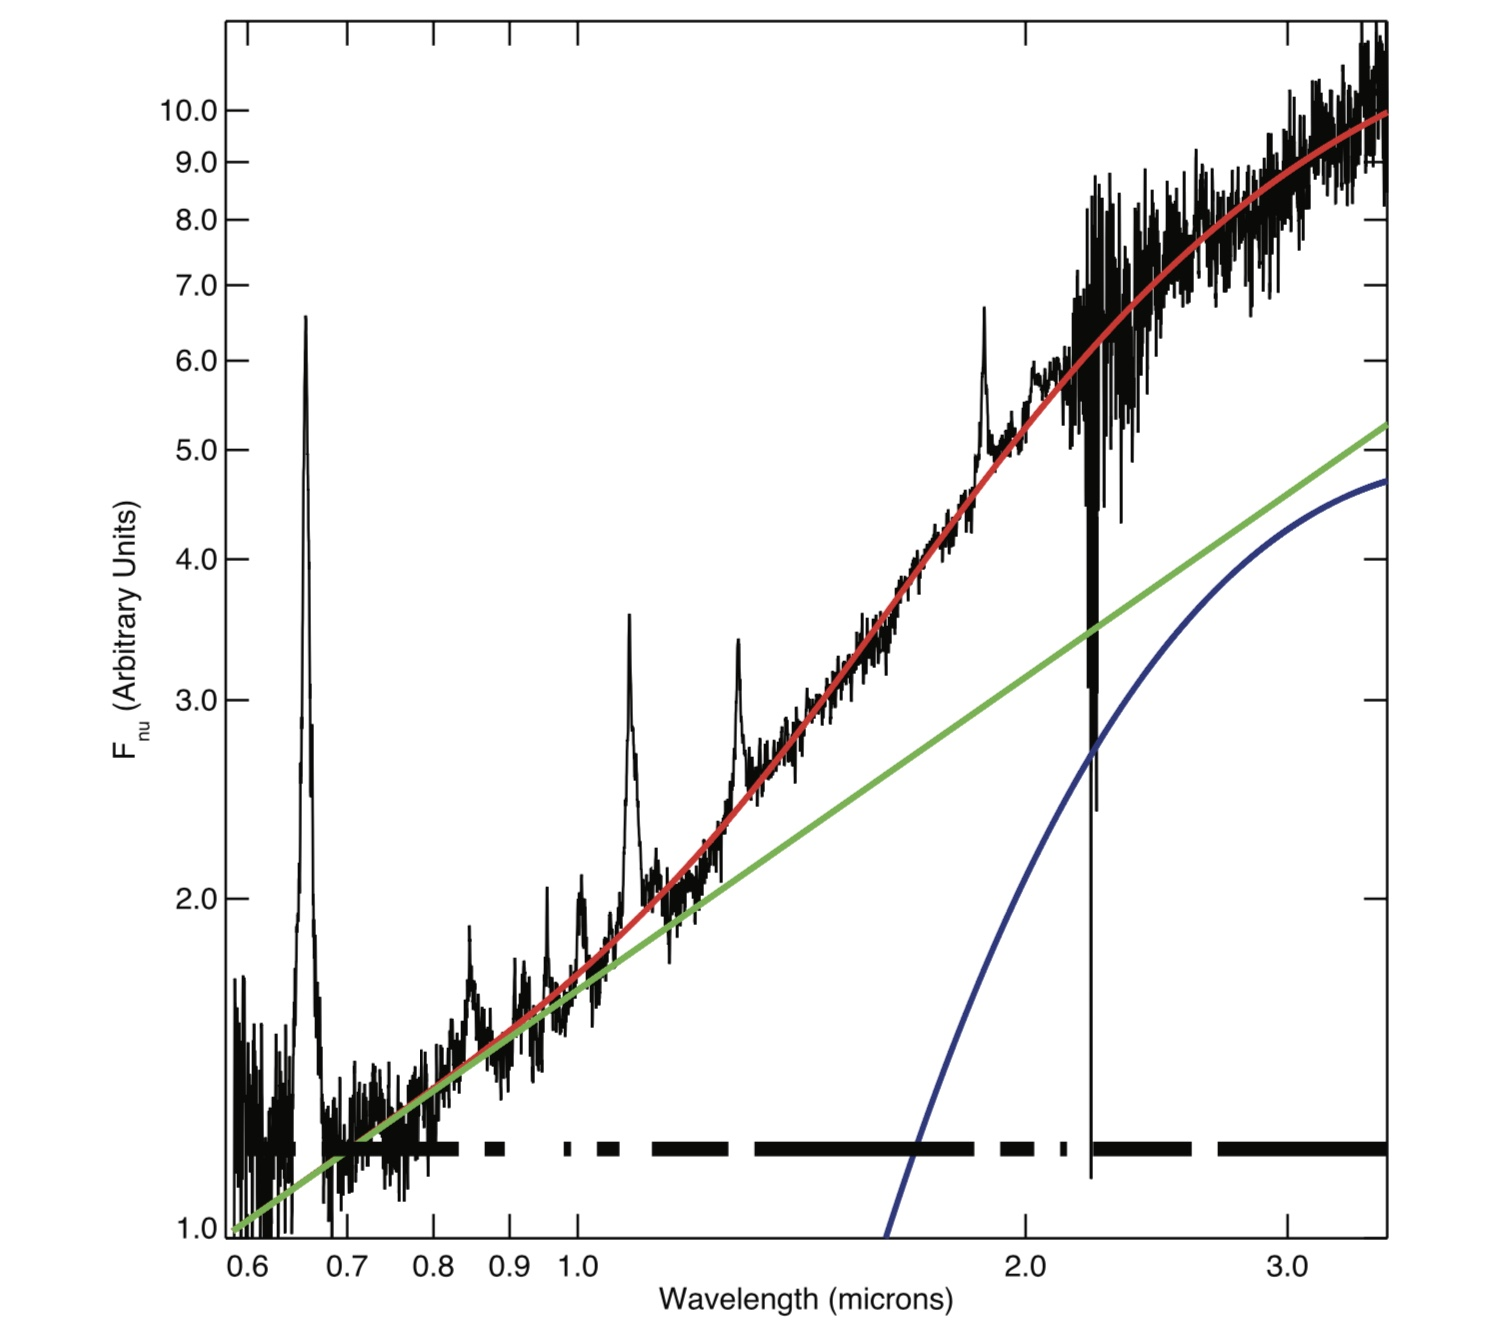
\includegraphics[width=\linewidth]{Glikman_2006_ApJ_640_579_Fig7.jpeg}\par 
    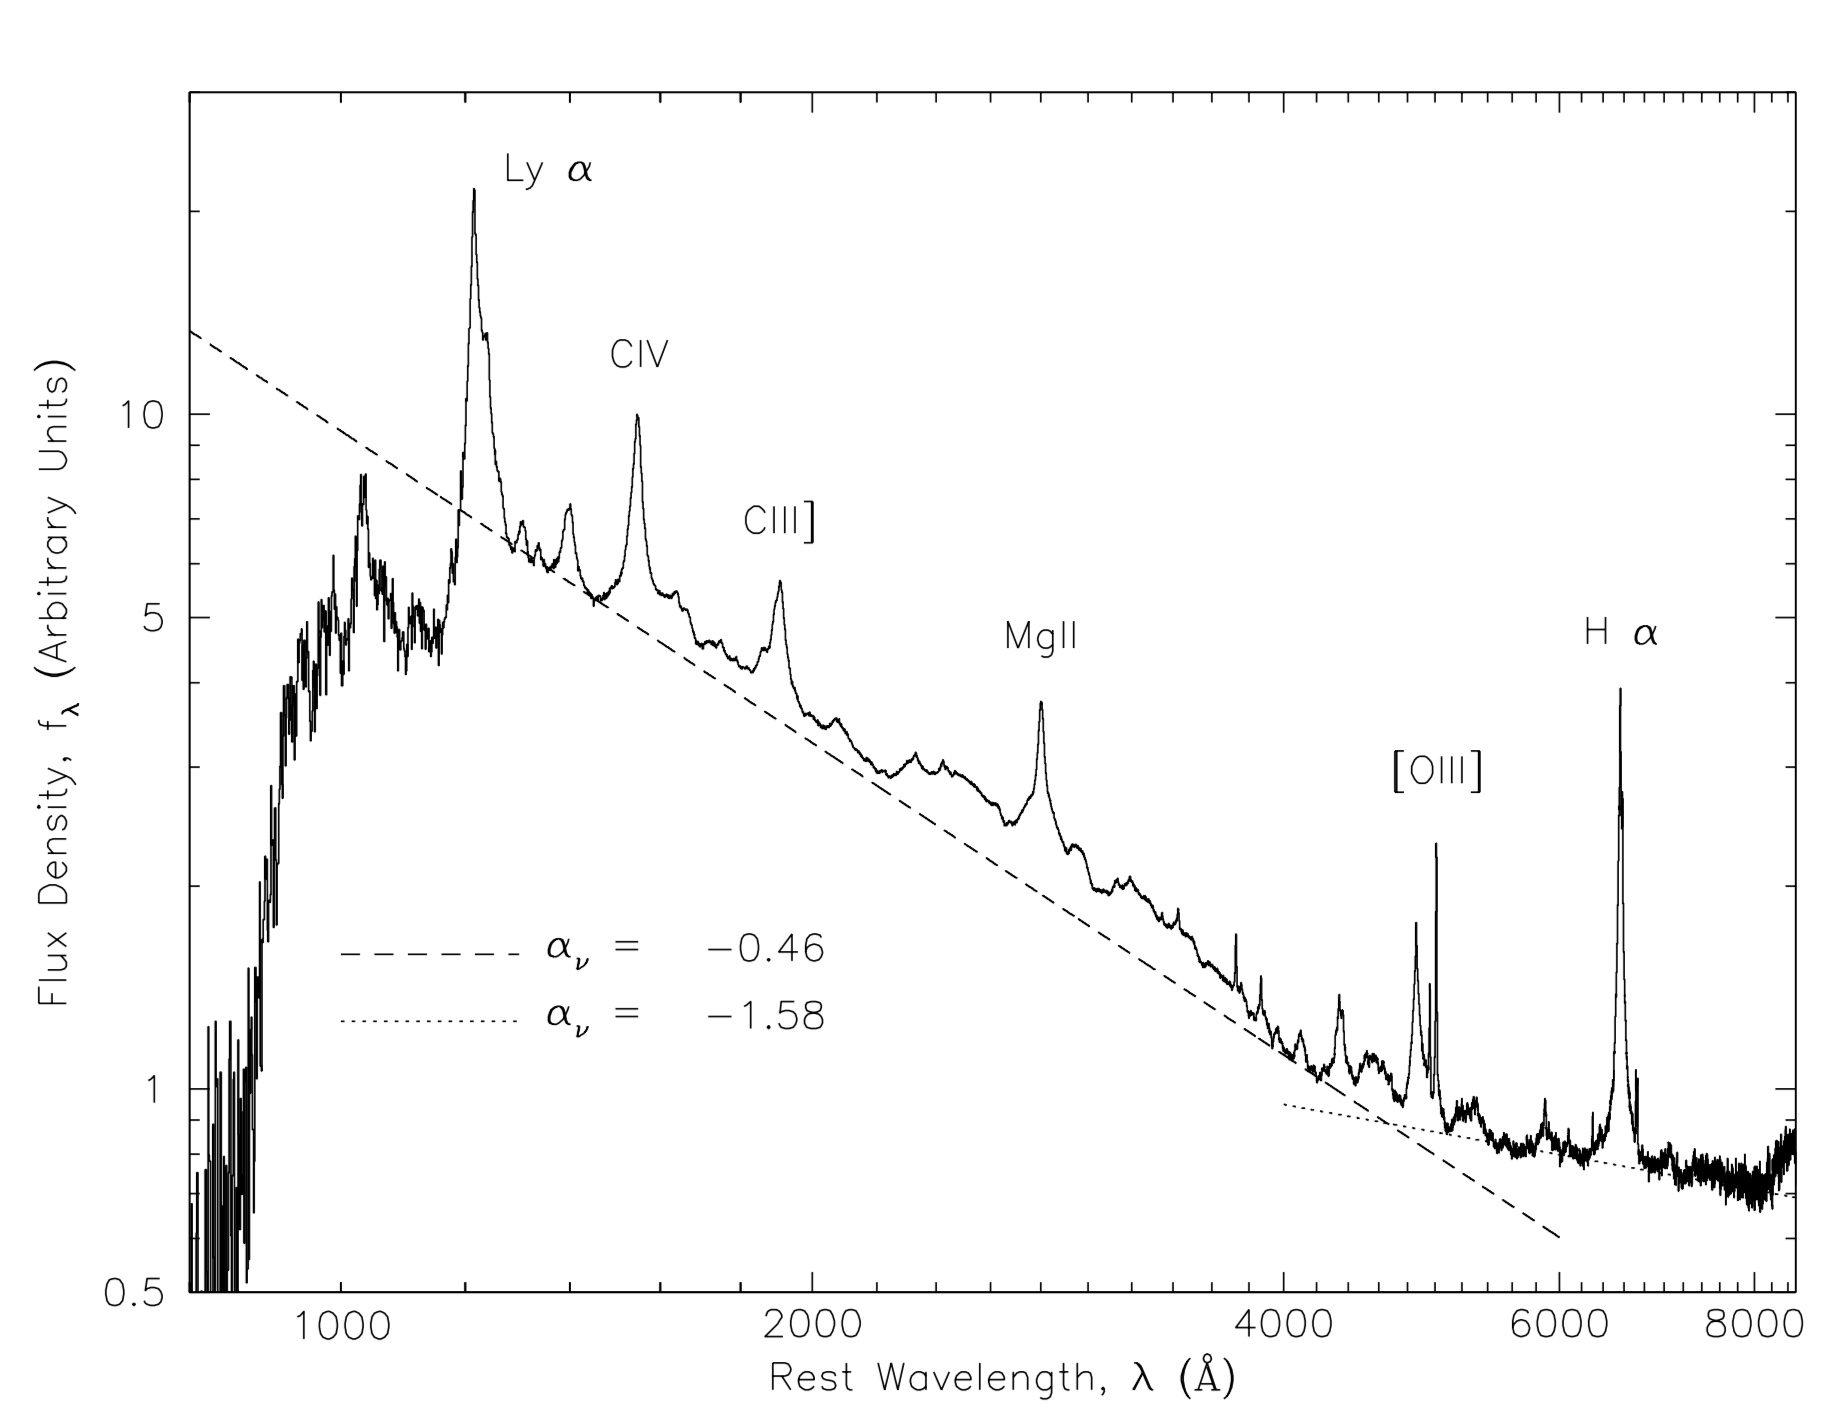
\includegraphics[width=\linewidth]{Vanden_Berk_2001_AJ_122_549_Fig3.jpeg}\par 
    \end{multicols}
\begin{multicols}{2}
    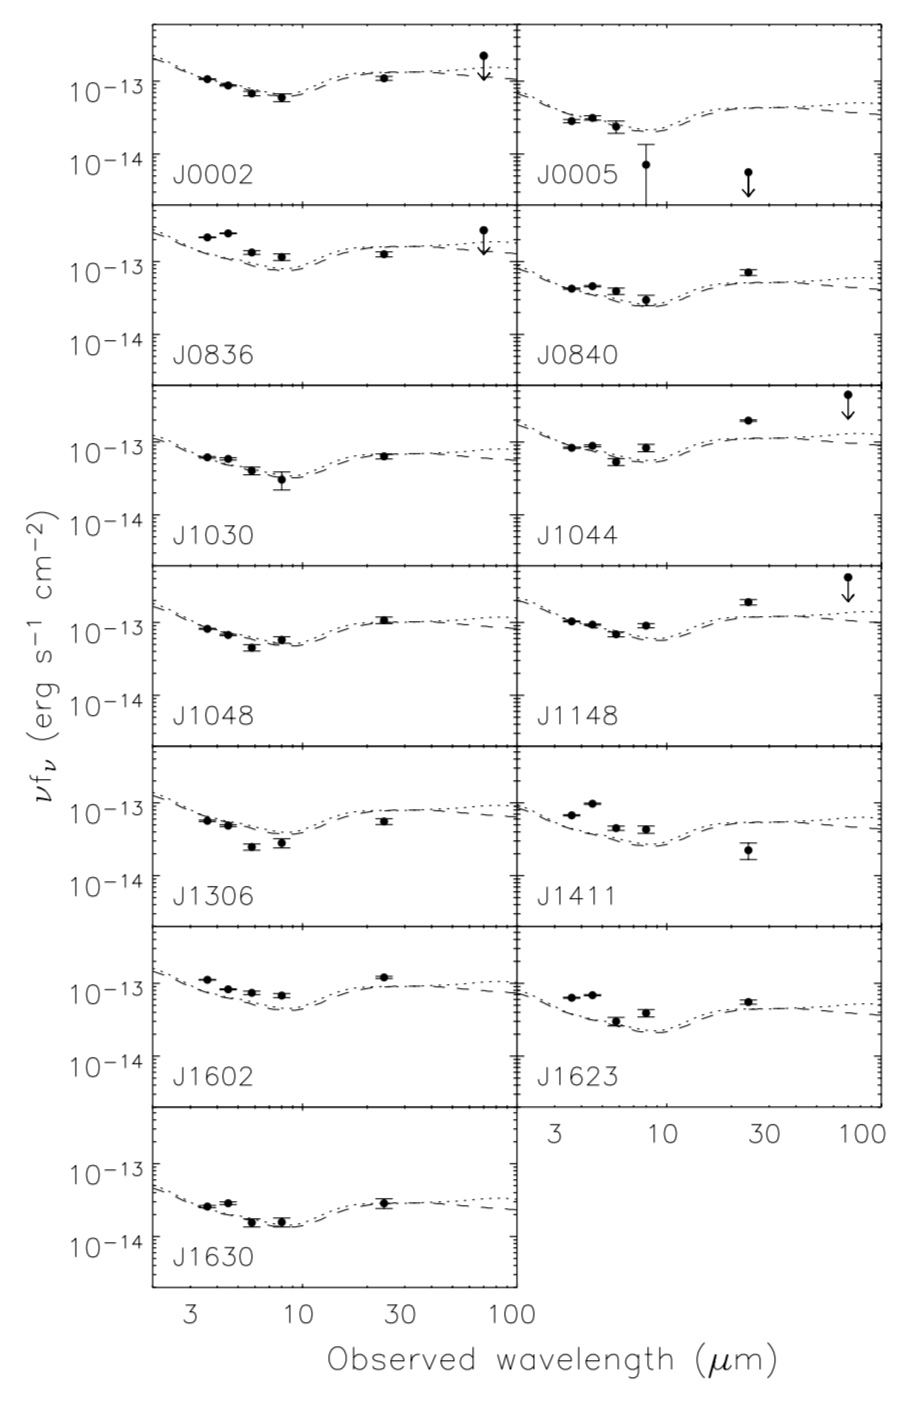
\includegraphics[width=\linewidth]{Jiang_2006_AJ_132_2127_Fig2.jpeg}\par
    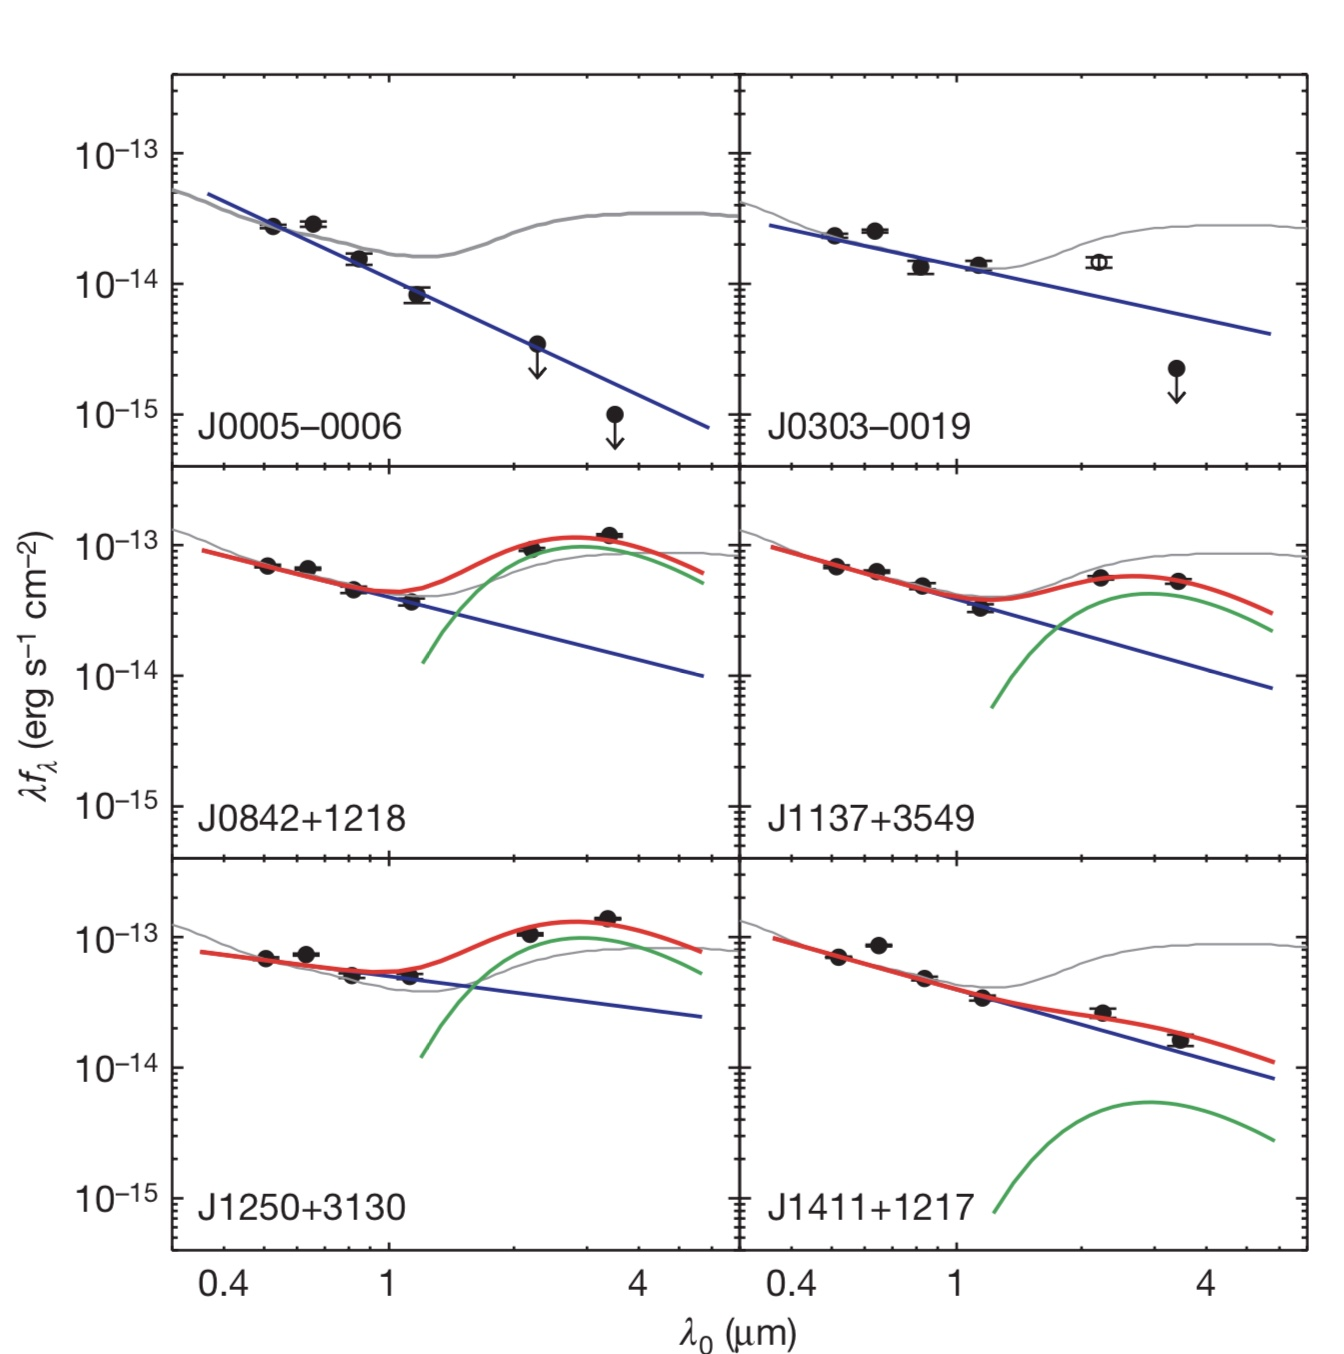
\includegraphics[width=\linewidth]{Jiang_2010_Nature_464_380_Fig1.jpeg}\par
\end{multicols}
    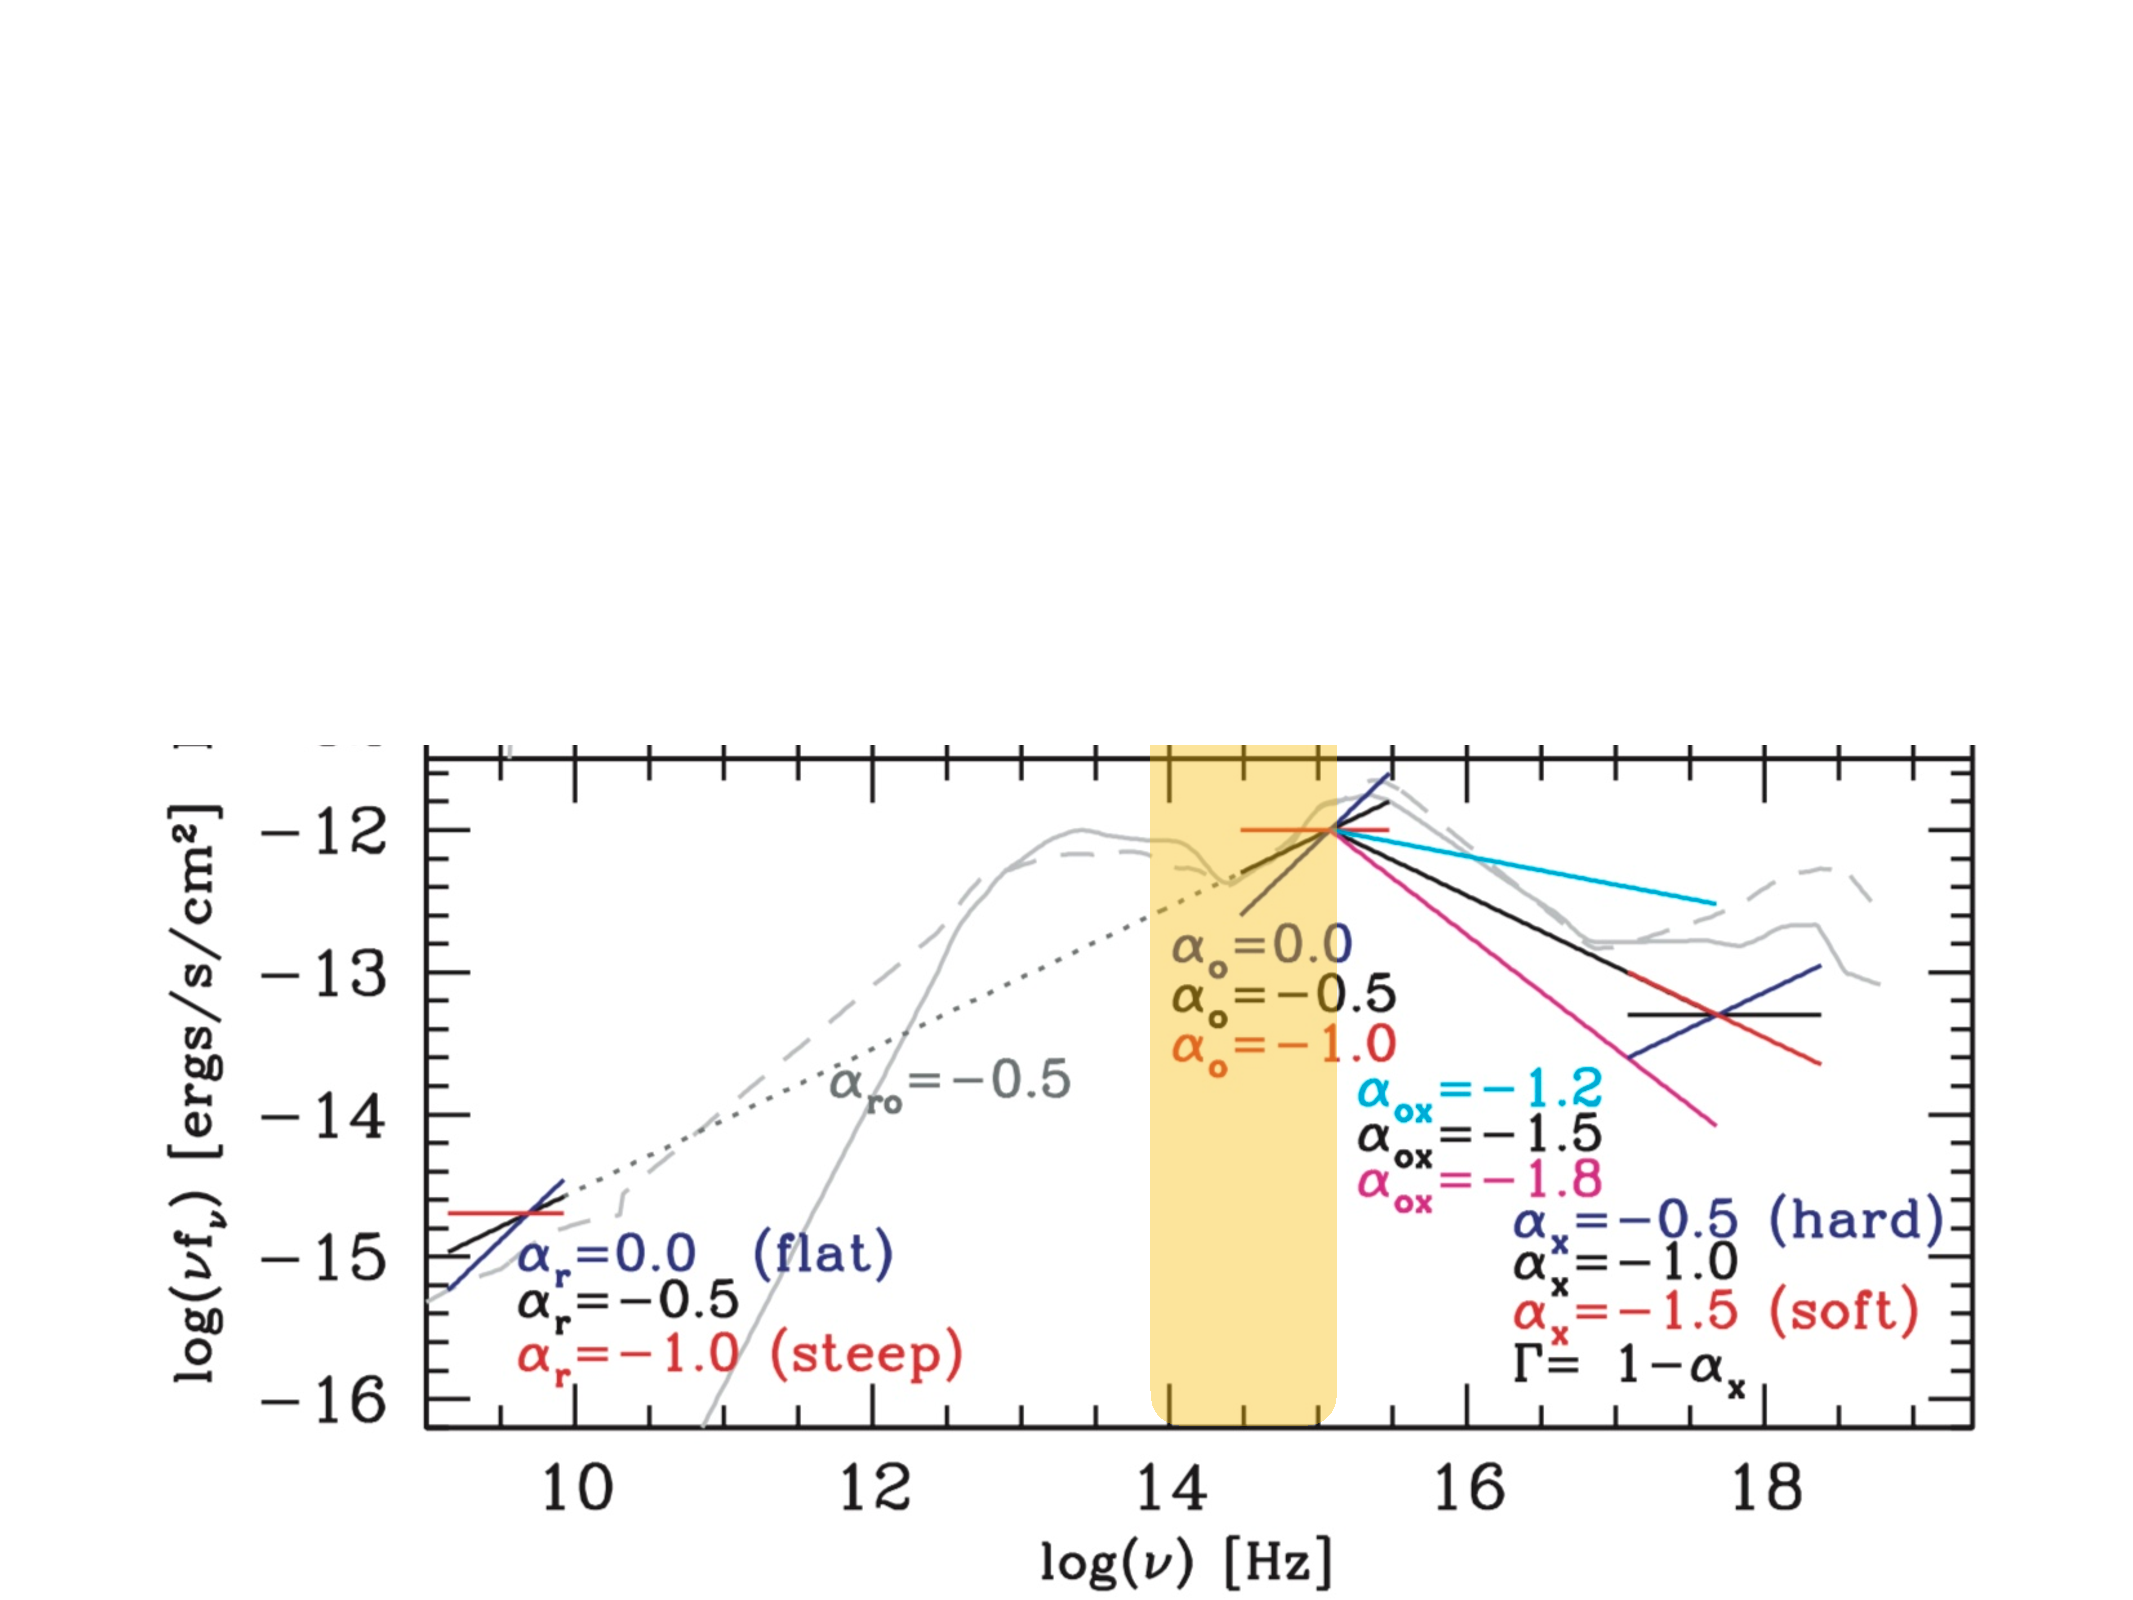
\includegraphics[width=\linewidth]{Richards_2006_ApJS_166_470_Fig10_bottomhalf.pdf}\par
\caption{
{\it Top Left:} Fig. 7 from \citet{Glikman2006}. $y$-axis is F$_{\nu}$; 
Power-law plus blackbody fit to their composite quasar spectrum plotted in F$_{\nu}$-$\lambda$ on logarithmic axes. 
The combined fit is shown in red, the power-law component with a best-fit spectral index of $\alpha_{\nu}=-0.92$ is shown in green, and the blackbody with the best-fit dust temperature of $T_{\rm dust}=1260$K  is shown in blue.\\
%%
{\it Top Right:} Fig. 3 from \citet{VdB2001}. $y$-axis is f$_{\lambda}$ Composite quasar spectrum using median combining. Power-law fits to the estimated continuum Ñux are shown. The resolution of the input spectra is $\approx$1800, which gives a wavelength resolution of about 1\AA\ in the rest frame. \\
%%
{\it Middle Left:} Fig. 2 from \citet{Jiang2006}. $y$-axis is $\nu$f$_{\nu}$.  SEDs of the 13 quasars from the {\it Spitzer} observations. The dotted and dashed lines represent the average SEDs of type I low-redshift quasars from Elvis et al. (1994) and Richards et al. (2006),  respectively, and have been normalized at rest frame 1450\AA\. Circles with downward arrows represent 2$\sigma$ upper limits. The measurement uncertainties are also given in the figure.\\
%%
{\it Middle Right:} Fig. 1 from \citet{Jiang2010}. $y$-axis is $\lambda$F$_{\lambda}$;  Spitzer SEDs of z < 6 quasars. Filled circles, rest-frame SEDs of six representative quasars from our sample in the four IRAC channels, the IRS PUI blue band (15.6$\mu$m) and the MIPS 24 $\mu$m band. 
Typical on-source integration time of the Spitzer observations was 10-30 min per source per band. The integration time for J0005-0006 at 15.6 and 24$\mu$m was about four hours and for J0303-0019 at 24$\mu$m was 50 min. The IRAC 4.5$\mu$m bandpass includes the strong H$\alpha$ emission line (6563) 
at this redshift, enhancing the flux. Open circle (in J0303-0019), problematic photometry due to contamination from heavily blended neighbours. Circles with downward arrows, 2$\sigma$ upper limits; error bars, measurement uncertainties (1$\sigma$). Grey lines, template formed from the average of a large number of low- redshift type 1 quasar SEDs, and normalized to each object at $\lambda$=3.6$\mu$m. Blue and green lines, respectively disk and hot-dust components from the best model fits (the IRAC data are used to fit the disk emission, and the IRS PUI and MIPS data are then used to constrain the hot dust emission); red lines, sum of the two. In J0005-0006 and J0303-0019, a power law is not a good description for the disk emission at $\lambda > 1\mu$m.\\
%%
{\it Bottom Row:} Bottom half of \citet{Richards2006b}, giving $\nu$f$_{\nu}$. Yellow box is $\sim$the wavelength coverage in the Jiang et al. plots. Shown in gray are the Elvis et al. (1994) radio-quiet (solid) and radio-loud (dashed) mean SEDs. The colored lines indicate typical spectral indices in the radio, optical, and X-ray using the same sign convention. Also shown is the typical radio-to-optical spectral index for radio-loud quasars and the range of optical–to–X-ray spectral indices. Studies in different bands tend to use different sign conventions for spectral indices and jargon to describe them (e.g., steep/red/soft). 
}
\end{figure*}



From Table~\ref{tab:units_overview}, to get from $L_{\nu}$ to $\nu L_{\nu}$, at say 1.0$\mu$m, you just have to multiply by
3$\times10^{14}$ (Hz), and this gives e.g. $\approx3\times10^{44}$ erg s$^{-1}$ :-) 

\begin{table}
  \begin{center}
    \setlength{\tabcolsep}{4pt}
    \begin{tabular}{lrrrl}
      \hline       \hline
      Unit Name   & Physical Quantity & symbos & Units     \\
      \hline
      Janksy & spectral flux density &  $f_{\nu}$ & $10^{-26}$ W                  m$^{-2}$ Hz$^{-1}$  \\
     Jansky  & spectral flux density &  $f_{\nu}$  & $10^{-23}$ erg s$^{-1}$ cm$^{-2}$ Hz$^{-1}$ \\
      \hline       \hline
    \label{tab:The_LRG_numbers}
    \end{tabular}
    \caption{e.g. Fig. 10 of Richards et al. (2006b).}
  \end{center}
\end{table}


\begin{eqnarray}
  m_{\rm AB} & =  & -2.5 \log_{10} \left(  \frac{f_{\nu}}{3631 \ {\rm Jy}} \right) \\
                 & =  & -2.5 \log_{10} \left(  \frac{f_{\nu}}{  {\rm Jy}} \right) + 8.90 \\
                 & =  &-2.5 \log_{10} f_{\nu} - 48.60 
\end{eqnarray}
with the -48.6 thing coming in if in $cgs$ units of erg s$^{-1}$ cm$^{-2}$ Hz$^{-1}$.\\

\noindent
So, with $\nu  f_{\nu}  = \lambda f_{\lambda}$, we can have: 
\begin{eqnarray}
  f_{\nu}              & = &  \frac{\lambda^{2}}{c} \ f_{\lambda}\\
\end{eqnarray}
Now, if $f_{\nu}$ is in Jansky's and $\lambda$ is in \AA\, then, 
$c$ must be in \AA\ s$^{-1}$, i.e.,  $c = 3\times10^{18}$ \AA\ s$^{-1}$.  
Then you just replace:
\begin{eqnarray}
%f_{\nu} & = & 1e23 \times \frac{\lambda^2}{c} f_{\lambda}\\
  f_{\nu}                      & = &  \frac{\lambda^{2}}{c} f_{\lambda}\\
  f_{\nu} {\rm (in\ Jy)} & = & 1  \times 10^{23}/(3e18) \ \frac{\lambda^{2}}{\AA} \ f_{\lambda}\\
  f_{\nu} {\rm (in\ Jy)} & = & 0.3 \times10^{5} \times \lambda^{2} \times f_{\lambda} \\ 
  f_{\nu} {\rm (in\ Jy)} & = & 3.34e4 \times \lambda^{2} \times f_{\lambda} \\
  \frac{f_{\nu}}{ [ {\rm Jansky} ] }  & = & 33,356 \left( \frac{\lambda}{ [ {\rm \AA} ] } \right)^{2} \frac{f_{\lambda}} {\rm erg s^{-1} cm^{-2}  \AA^{-1}} 
\end{eqnarray}
with 1 cm being 1$\times10^{8}$\AA\ and $c=2.99792\times10^{10}$ cm s$^{-1}$. \\

\noindent
Following e.g. URL [5], 
\begin{eqnarray}
f_{\nu}                      & = & A \times \lambda f_{\gamma}\\
f_{\nu} {\rm (in\ Jy)} & = & 6.626\times10^{-8} \frac{\lambda}{[\mu m]} f_{\gamma}\\
\end{eqnarray}
where $f_{\nu}$ is the `energy flux', aka the spectral flux density,
measured in Janskys (10$^{-26}$ W m$^{-2}$ Hz$^{-1}$), $f_{\gamma}$ is
the `photon flux' measured in s$^{-1}$ m$^{-2}$ $\mu$m$^{-1}$,
$\lambda$ is the wavelength measured in $\mu$m and Planck's constant
is 6.626$\times10^{-34}$ m$^{2}$ kg s$^{-1}$ (i.e. 6.626e-34*1e26 =
6.626e-8).\\

\noindent
Take your $f_{\nu}$ measurements that are in Jy. (Ensure they are in
Jy! If they're in magnitudes, convert them to Jy first; see
'magnitude' discussion above.) Multiply by $1\times10^{-23}$ to get
them into {\it cgs} units. Multiply these $f_{\nu}$ values by
$\frac{c}{\lambda^{2}}$ to get them into $f_{\lambda}$. Multiply them
by $\lambda$ to get them into $\lambda f_{\lambda}$. WATCH YOUR
UNITS. NB: $c = 2.997924\times10^{10}$ cm sec$^{-1}$. \\

\noindent
Also note/recall, 
\begin{equation}
  \nu  f_{\nu}    =  \lambda  f_{\lambda}
\end{equation}
with units of ergs s$^{-1}$ cm$^{-2}$. 

\subsection{Assef et al. 2010}
To go from Table 1 (F$_{\nu}$ in erg s$^{-1}$ cm$^{-2}$ Hz$^{-1}$) to Figure 3 (with y-axis $\nu$ F$_{\nu}$) I did:: 

\begin{lstlisting}
lam = wave * 1e-6
nu = 3e8/lam
ax1.plot(Assef_wave, Assef_AGN*nu*1e-17,  color='black')
ax2.plot(Assef_wave, Assef_E   *nu *1e-19,   color='red')
ax3.plot(Assef_wave, Assef_Sbc *nu *4e-20,  color='green')
ax4.plot(Assef_wave, Assef_Im  *nu *1e-19,   color='cyan')

## Noting the 1e-17,  1e-19, 4e-20 and 1e-19 factors here 
## are 'completely' arbitary and just to get things on the 
## same plot...
\end{lstlisting}


\section{Unit Conversions}
    \subsection{Flux density to AB}
    The flux density in Jy can be converted to a magnitude basis:\\
    (straight from Wiki!! ;-):\\
    \begin{eqnarray}
      S_{\nu} [\mu {\rm Jy} ]  & = & 10^{6} \cdot 10^{23} \cdot 10^{-{{\rm AB} +48.6/2.5 }} \\
                                        & = & 10^{(23.9 - {\rm AB})/2.5} \\
    \end{eqnarray}

%% https://en.wikipedia.org/wiki/Luminosity



\section{WISE}
The source flux density, in Jansky [Jy] units, is computed from the calibrated WISE (Vega) magnitudes, $m_{\rm Vega}$ using:
N.B the WISE webpage (given in the URL notes below) uses $F_{\nu}$ for source flux density. I'm going to stick with my convention and use little $f$, $f_{\nu}$, 
\begin{equation}
  f_{\nu} [{\rm Jy}]  =  f_{\nu, 0} \times 10^{(-m_{\rm Vega}/2.5)} 
\end{equation}
where $f_{\nu, 0}$ is the zero magnitude flux density corresponding to the constant that gives the same response as that of Alpha Lyrae (Vega). For most sources, the zero magnitude flux density, derived using a constant power-law spectra, is appropriate and may be used to convert WISE magnitudes to flux density [Jy] units. Table 1 lists the zero magnitude flux density (column 2) for each WISE band.\\

\noindent
For sources with steeply rising MIR spectra or with spectra that deviate significantly from $f_{\nu}=$constant, including cool asteroids and dusty star-forming galaxies, a color correction is required, especially for W3 due to its wide bandpass. With a given flux correction, $f_{c}$, the flux density conversion is given by:
\begin{equation}
  f_{\nu} [{\rm Jy}]  = (f^{*}_{\nu, 0}/f_{c}) \times 10^{(-m_{\rm Vega}/2.5)} 
\end{equation}
where $f^{*}_{\nu, 0}$ is the zero magnitude flux density derived for sources with power-law spectra: $f_{\nu} \propto \nu^{2}$, listed in Table 1 (column 3) and the flux correction, $f_{c}$, listed in Table 2 for $f_{\nu} \propto \nu^{-\alpha}$, where the index $\alpha$  ranges from: -3, -2, -1, 0, 1, 2, 3, and 4, and for blackbody spectra, B$_{\nu}$(T) for a variety of temperatures, and for stars of two main-sequence spectral types (K2V and G2V). 




\section{Links}
Some of these are old/broken... :-( \\

%% Using \\ and square brackets seems to crash with [2] !!
\noindent
[1] \href{http://www.iasf-milano.inaf.it/$\sim$polletta/templates/images/new\_Arp220\_template.jpg}{http://www.iasf-milano.inaf.it/$\sim$polletta/templates/images/new\_Arp220\_template.jpg}

\noindent
[2] \href{http://www.astro.soton.ac.uk/$\sim$td/flux\_convert.html}{http://www.astro.soton.ac.uk/$\sim$td/flux\_convert.html}

\noindent
[3] \href{http://coolwiki.ipac.caltech.edu/index.php/Units}{http://coolwiki.ipac.caltech.edu/index.php/Units}

\noindent
[4] \href{http://wise2.ipac.caltech.edu/docs/release/allsky/expsup/sec4\_4h.html}{http://wise2.ipac.caltech.edu/docs/release/allsky/expsup/sec4\_4h.html}

\noindent
[5] \href{http://www.astro.ljmu.ac.uk/~ikb/convert-units/node1.html}{http://www.astro.ljmu.ac.uk/~ikb/convert-units/node1.html}

\noindent
[6] \href{http://xingxinghuang.blogspot.co.uk/2013/06/hello-everybody-if-you-still-get.html}{http://xingxinghuang.blogspot.co.uk/2013/06/hello-everybody-if-you-still-get.html}

\noindent
\href{http://ssb.stsci.edu/doc_tmp/stsci_python_dev/pysynphot.doc/html/units.html}{http://ssb.stsci.edu/doc\_tmp/stsci\_python\_dev/pysynphot.doc/html/units.html}

\noindent
\href{http://www.stsci.edu/~strolger/docs/UNITS.txt}{http://www.stsci.edu/$\sim$strolger/docs/UNITS.txt}

\noindent
\href{https://github.com/spacetelescope/pysynphot/blob/master/doc/source/units.rst}{https://github.com/spacetelescope/pysynphot/blob/master/doc/source/units.rst}

\noindent
\href{https://www.astro.umd.edu/~ssm/ASTR620/mags.html}{https://www.astro.umd.edu/$\sim$ssm/ASTR620/mags.html}



\bibliographystyle{mn2e}
%\bibliography{tester_mnras}
\bibliography{/cos_pc19a_npr/LaTeX/tester_mnras}



\end{document}

